\subsection{Optimierung}
%\label{subsection:Optimierung}
Im Projekt wurden drei Optimierungen vorgenommen, um die Laufzeit zu verkürzen.\\

\subsubsection{Optimierungsschritt}
Um die Laufzeit des Programms zu verkürzen, werden nicht mehr die einzelnen Chars, die ein Wort bilden verschickt, sondern ein Array  mit allen Chars bzw. Wörtern zusammengesetzt. Um zu verdeutlichen aus welchen Chars ein Wort besteht, wird zwischen den Wörter ein Semikolon eingefügt. Dadurch kann der Slave das Array nach den Wörtern aufteilen. Dies führt zu einer Optimierung der Laufzeit, da die Befehle von \textit{MPI\_Send()} und \textit{MPI\_Recv()} nicht mehr nach jedem Char ausgeführt werden sondern nur noch einmal pro Prozess. \\
Wenn die Chars aus der einzulesenden Datei einzeln verschickt werden, sind es ca. 2.465.500 Aufrufe der Funktionen \textit{MPI\_Send()} und \textit{MPI\_Recv()}. Zusätzlich werden auch beim Rücksenden der einzelnen Zeichen an den Master ca. 2.465.500 Aufrufe der beiden Funktionen benötigt.\\
Nach der Optimierung waren Verbesserungen der Laufzeit zu beobachten. Zwei Prozesse benötigten nun insgesamt 2,5 Sekunden zum Sortieren. Vor der Optimierung lag die Laufzeit bei vier Prozessen zum Vergleich bei etwa 3 Sekunden.  

\subsubsection{Optimierungsschritt}
Im ersten Programmentwurf versendet der Master die Wörter an die sieben Prozesse zum Sortieren, ohne selber einen Bereich zu sortieren. Dies führt dazu, dass ein Prozess nur die Daten verschickt und empfängt. In der Zwischenzeit, wo die sieben Prozesse sortieren, wartet ein Prozess bis Daten zurückgeschickt werden. Diese Zwischenzeit kann der Master nutzen, um selber einen Teilbereich zu sortieren. So werden acht statt sieben Prozesse zum Sortieren genutzt.  

\subsubsection{Optimierungsschritt}
Eine weiterer Optimierungsschritt ist, dass alle eingelesenen Wörter aus der Datei in einem Array verschickt werden. Somit muss der Array zunächst nicht in die einzelnen zu sortierenden Bereiche aufgeteilt werden. Jeder Prozess erhält einen Buchstabenbereich von 2-3 Buchstaben. Z.B. erhält der erste Prozess den Buchstabenbereich von a und b. Somit sortiert er nur die Wörter alphabetisch, die mit a oder b anfangen. Die Optimierung liegt am Zusammenführen der einzeln sortierten Arrays der Slaves. Der Master fügt die sortierten Arrays hintereinander zu einem vollständig Array zusammen, in dem alle Wörter enthalten sind. \\

%Mögliche Optimierung (wenn nicht gewünscht weglassen)
\subsection{Optimierter Algorithmus}
Zusätzlich zu den Optimierungen am bestehenden Algorithmus wird eine alternative Aufteilung und Sortierung der Daten erarbeitet. Anstatt den initial Vektor auf einer Master Node auf eine unbestimmte Anzahl Worker aufzuteilen, kann eine Baumstruktur erstellt werden. Dabei sendet eine Ursprungsnode die Hälfte des Datensatzes an eine weitere Node. Diesen Prozess setzt jede Node unabhängig fort, bis alle Worker verwendet werden. Nun führt jeder Worker den Merge-Sort durch und sendet den sortierten Vektor wieder an die Node, von welcher er den Vektor erhalten hat. Diese Node führt nun durch die bestehende Funktion des Merge-Sorts die beiden sortierten Vektoren in einen sortierten Vektor zusammen und sendet diesen wiederum an die Node, von welcher die unsortierten Daten gesendet wurden. Dieser Prozess wird so lange wiederholt, bis die Ursprungsnode wieder die gesamten Daten hat. Das Ergebnis ist ein sortierter Vektor. Es werden hierbei nicht nur die Sortierungen Parallelisiert, sondern auch das Versenden der Daten, sowie das Zusammenführen der Daten. Die gleichzeitige Ausführung von mehreren Prozessen sorgt dabei für eine bessere Ausnutzung der verfügbaren Rechenkapazität. Aufgrund von mangelnder Zeit wurde dieser Algorithmus im Rahmen dieser Arbeit nicht implementiert und getestet.
\begin{figure}[!t]
	\centering
	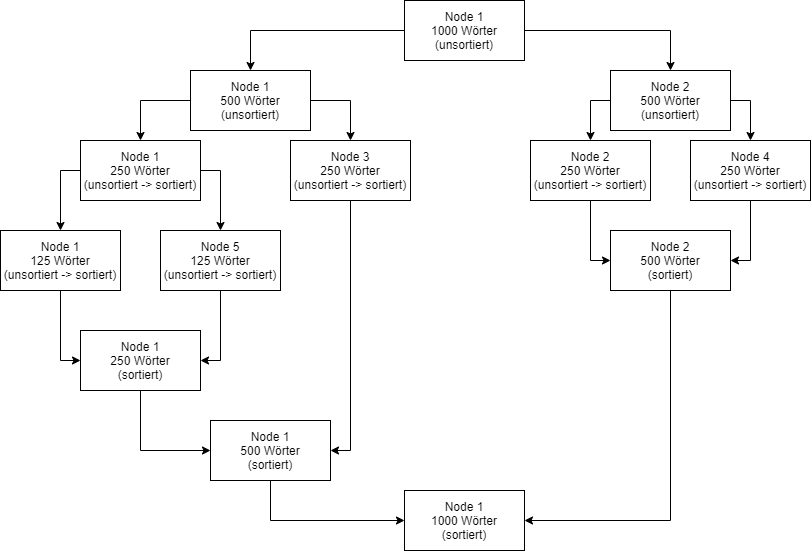
\includegraphics[width=3.5in]{Parallelisierungs_Algorithmus_2.png}
	\caption{Beispielhafter Durchlauf des Algorithmus mit 5 Nodes}
	\label{para_algo2}
\end{figure}